%% Final edits by Kai Puolamäki, based on the Data Science template.
%% Final edits by Jussi Kangasharju and Pirjo Moen
%% This file is modified by Veli Mäkinen from HY_fysiikka_LuKtemplate.tex authored by Roope Halonen ja Tomi Vainio.
%% Some text is also inherited from engl_malli.tex by Kutvonen, Erkiö, Mäkelä, Verkamo, Kurhila, and Nykänen.


% STEP 1: Choose oneside or twoside
\documentclass[english,twoside,openright]{UH_TCM_MSc}
%finnish,swedish

\usepackage{lmodern} % Font package
\usepackage{textcomp} % Package for special symbols
\usepackage[pdftex]{color, graphicx} % For pdf output and jpg/png graphics
\usepackage[pdftex, plainpages=false]{hyperref} % For hyperlinks and pdf metadata
\usepackage{fancyhdr} % For nicer page headers
\usepackage{tikz} % For making vector graphics (hard to learn but powerful)
%\usepackage{wrapfig} % For nice text-wrapping figures (use at own discretion)
\usepackage{amsmath, amssymb,amsfonts,amssymb,amscd} % For better math
%\usepackage[square]{natbib} % For bibliography
\usepackage[footnotesize,bf]{caption} % For more control over figure captions
\usepackage{blindtext}
\usepackage{titlesec}
\usepackage[titletoc]{appendix}
\usepackage{svg}
\usepackage{subcaption}
\usepackage{mathrsfs}
\usepackage{cancel}
\usepackage{bbm}
\usepackage{algorithmic}
%\usepackage{babel}
\usepackage[en-GB]{datetime2}


\onehalfspacing %line spacing
%\singlespacing
%\doublespacing

%\fussy 
\sloppy % sloppy and fussy commands can be used to avoid overlong text lines

% STEP 2:
% Set up all the information for the title page and the abstract form.
% Replace parameters with your information.
\title{$SU(N)$ Gauge Theory With a Twist: Measuring the Tension between two ordered phases in Pure $SU(N)$ Gauge Theory}
\author{Aaron Haarti}
\date{\today}
\prof{Professor Kari Rummukainen}
\censors{Professor Y}{Dr. Z}{}
\keywords{layout, summary, list of references}
\depositeplace{}
\additionalinformation{}

% Comment the following lines if you do not want the ACM classification.
\classification{\protect{\ \\
\  General and reference $\rightarrow$ Document types  $\rightarrow$ Surveys and overviews\  \\
\  Applied computing  $\rightarrow$ Document management and text processing  $\rightarrow$ Document management $\rightarrow$ Text editing\\
}}

% if you want to quote someone special. You can comment the line, and nothing will be on the document.
%\quoting{Bachelor's degrees make pretty good placemats if you get them laminated.}{Jeph Jacques} 


% OPTIONAL STEP: Set up properties and metadata for the pdf file that pdfLaTeX makes.
% But you don't need to do this unless you want to.
\hypersetup{
    %bookmarks=true,         % show bookmarks bar first?
    unicode=true,           % to show non-Latin characters in Acrobat’s bookmarks
    pdftoolbar=true,        % show Acrobat’s toolbar?
    pdfmenubar=true,        % show Acrobat’s menu?
    pdffitwindow=false,     % window fit to page when opened
    pdfstartview={FitH},    % fits the width of the page to the window
    pdftitle={},            % title
    pdfauthor={},           % author
    pdfsubject={},          % subject of the document
    pdfcreator={},          % creator of the document
    pdfproducer={pdfLaTeX}, % producer of the document
    pdfkeywords={something} {something else}, % list of keywords for
    pdfnewwindow=true,      % links in new window
    colorlinks=true,        % false: boxed links; true: colored links
    linkcolor=black,        % colour of internal links
    citecolor=black,        % colour of links to bibliography
    filecolor=magenta,      % colour of file links
    urlcolor=cyan           % colour of external links
}

\DeclareMathOperator{\Tr}{Tr}
\DeclareMathOperator{\z}{\mathbf{z}}
\newcommand{\id}{\mathbbm{1}}

\begin{document}

% Generate title page.
\maketitle

% STEP 3:
% Write your abstract (of course, you do this last).
% You can make several abstract pages (if you want it in different languages),
% but you should also then redefine some of the above parameters in the proper
% language as well, in between the abstract definitions.

\begin{abstract}
something something SU(N)
\end{abstract}

% Place ToC
\mytableofcontents

\mynomenclature

% -----------------------------------------------------------------------------------
% STEP 4: Write the thesis.
% Your actual text starts here. You shouldn't mess with the code above the line except
% to change the parameters. Removing the abstract and ToC commands will mess up stuff.
\chapter{Introduction}

Introduce the main concepts of the theory and the boundary condition that imposes the physics. Then introduce the tools and technology used to measure the surface and analyse the system including error analysis techniques. Monte Carlo sampling techniques, Jackknife, FS reweighting etc. Lastly talk about results found from the measurements

\chapter{Constructing SU(N) Gauge Theory on the Lattice} \label{ch:sun_gauge_theory}

\section{Pure SU(3) Gauge Theory on the Lattice: Motivation and construction of the Gauge action}

In this section we will follow closely the lecture notes of Christof Gattringer and Christian B. Lang \cite[ch.~2]{gattringer2009quantum}. To begin the understanding of gauge theories on the lattice, it is useful to start from a well known theory which is more or less grounded in reality. $SU(3)$ gauge theory, also known as Quantum Chromodynamics (QCD), is a theory which has been well established in the standard model of physics and is the fundamental theory for the strong interaction between quarks and gluons. This theory holds a substantial amount of mathematical structure, and complexities arise especially when the theory begins to describe the relationship of quark fields in the QCD action. Since we are only interested in pure $SU(N)$ gauge theory, meaning the aspect of the theory which mediates the interaction between the quark fields, we will keep our focus on the gluon fields.

The gluon fields, also known as the gauge fields can be described with the following form \cite[p.~26]{gattringer2009quantum}:
\begin{align}
    A_\mu(x)_{cd},
\end{align}
where the argument $x$ describes a location in space time while the Lorentz index $\mu = 1,2,3,4$ holds our direction in space time for our vector field. For each location $x$ and index $\mu$ the element $A_\mu(x)$ is represented with a traceless Hermitean $3\times 3$ matrix, this is an important note which we will discuss more later. Since we are interested in the Euclidian action the index $\mu$ is also Euclidian, meaning that the notion of covariant and contravariant indices are dismissed. We will discuss the reasoning for this when we approach the path integral. Lastly we have color indices tied to the gluons $c,d = 1,2,3$.

As was stated before, our main focus is the gauge field, but since it's symmetries aren't completely decoupled from the Fermion fields, we need to direct our focus for a moment towards the full QCD action. Taking inspiration from electrodynamics we require similar invariance for the QCD action, where in the action is invariant under multiplication of fermion fields with an arbitrary phase factor which in turn implies a transformation for the gauge fields. Similarly in QCD we require invariance under local rotation of the color indicies and the consequential transformation of the gauge field. Let $\psi(x)$ be a fermion field, thus we require the action to be invariant under the following transformations \cite[p.~28]{gattringer2009quantum}:
\begin{align}
    \psi(x) \rightarrow \psi'(x) &= \Omega(x)\psi(x) \\
    \Bar{\psi}(x) \rightarrow \Bar{\psi}'(x) &= \Bar{\psi}(x)\Omega^\dagger(x) \\
    S[\psi(x),\Bar{\psi}(x),A_\mu(x)] &= S[\psi'(x),\Bar{\psi}'(x),A'_\mu(x)].
\end{align}
The elements $\Omega(x)$ which are responsible for rotating the color indices are defined to be $3\times 3$ complex matrices which obey the following definitions:
\begin{align}
    \det[\Omega(x)] &= 1 \\
    \Omega(x)^\dagger &= \Omega(x)^{-1}, \label{eq:2.6}
\end{align}
the latter definition tells us that the matrices are unitary. Both of these requirements are charachteristic definition of the special unitary group hence $\Omega \in SU(3)$. Some important characteristics of any group are that the identity element is required to exist in the set of group elements, the elements are closed under multiplication and that for each element there exists an inverse. Additionally $SU(3)$ is a non abelian group, meaning that the group elements do not commute $\Omega_x,\Omega_y \in SU(3) \Rightarrow [\Omega_1,\Omega_2]\neq \delta_{xy}$. With these rules in mind we can solve the gauge transformation implied by the fermionic action invariance:
\begin{align}
    \hspace{36px}S[\psi(x),\Bar{\psi}(x),A_\mu(x)] = S[\psi'(x),\Bar{\psi}'(x),A'_\mu(x)]
\end{align}
\begin{align}
     \iff \int d^4x \Bar{\psi}(x)&(\gamma_\mu(\partial_\mu + iA_\mu(x)) + m)\psi(x)  = \\
     &\int d^4x \Bar{\psi}(x) \Omega^\dagger(x)(\gamma_\mu(\partial_\mu + iA'_\mu(x)) + m)\Omega(x)\psi(x),
\end{align}
it is obvious that the mass term is equivalent on both sides due to the inverse nature \ref{eq:2.6}. The first term is more complicated. The structure of the $\gamma_\mu$ matrices, while being very important in QCD are less so in our case, thus we can disregard their structure and simply note that they freely commutes with the group elements $\Omega(x)$, hence we get the following relation:
\begin{align}
    (\partial_\mu + iA_\mu(x)) &= \Omega^\dagger(x)(\partial_\mu + iA'_\mu(x))\Omega(x) \label{eq:2.10} \\ 
    &= \Omega^\dagger(x)\Omega(x)\partial_\mu + \Omega^\dagger(x)[\partial_\mu\Omega(x)] + i\Omega^\dagger(x)A'_\mu(x)\Omega(x) \\ 
    &= \partial_\mu + \Omega^\dagger(x)[\partial_\mu\Omega(x)] + i\Omega^\dagger(x)A'_\mu(x)\Omega(x),
\end{align}
above we used the product rule for the first term due to the fact that the operator is acting on an implied function dependent on $x$. Let us then rearrange and solve for $A'_\mu(x)$ yielding the transformation rule as:
\begin{align}
    A_\mu(x) \rightarrow A'_\mu(x) = \Omega(x)A_\mu(x)\Omega(x)^\dagger + i[\partial_\mu\Omega(x)]\Omega^\dagger(x). \label{eg:2.13}
\end{align}

We stated earlier that the gauge field elements are required to be traceless and Hermitean, thus we must ask if the transformed gauge field holds these properties. First let's question the Hermitean nature of the transformation. We will take the following result directly from the appendix in Gattringer and Lang \cite[p.~329 A.1.4]{gattringer2009quantum} where the general discussion is on the derivative of group elements $\Omega$ :
\begin{align}
    -i\Omega(x)[\partial_\mu\Omega^\dagger(x)] = i[\partial_\mu\Omega(x)]\Omega^\dagger(x),
\end{align}
with this result we can directly show the Hermitean requirement, keeping in mind that $A_\mu$ is defined as Hermitean:
\begin{align}
    A_\mu^{'\dagger}(x) &= \Omega(x)A^\dagger_\mu(x)\Omega(x)^\dagger-i\Omega(x)[\partial_\mu\Omega^\dagger(x)] \\
    &= \Omega(x)A_\mu(x)\Omega(x)^\dagger + i[\partial_\mu\Omega(x)]\Omega^\dagger(x) = A'_\mu(x),
\end{align}
thus the transformed gauge field is Hermitean. Next we must ask if it is traceless, for which the first term is simple enough. $A_\mu$ is defined to be traceless hence:
\begin{align}
    \Tr[\Omega(x)A_\mu(x)\Omega(x)^\dagger] = \Tr[\Omega(x)^\dagger\Omega(x)A_\mu(x)] = \Tr[A_\mu(x)] = 0.
\end{align}
The second term is a bit more involved, but on line (A.14) of the aforementioned appendix it is shown that the second term is in fact also traceless.  We have show that our recovered result for the gauge transformation preserve the definitions of the gauge field. 

With the knowledge of the imposed gauge transformation produced by the symmetries defined for the fermion field we can move our focus towards the gluon action. The gluon action is a functional dependent of the gluon fields which is invariant under the transformation \ref{eg:2.13}:
\begin{align}
    S_G[A'] = S_G[A].
\end{align}
To construct this action we must first define a covariant derivative:
\begin{align}
    D_\mu = (\partial_\mu + iA_\mu(x)),
\end{align}
which based on line \ref{eq:2.10} transforms in the following manner:
\begin{align}
    D_\mu \rightarrow D'_\mu = \Omega(x)D_\mu\Omega^\dagger(x),
\end{align}
looking for a moment at the action transformation, the covariant derivative and it's transformation ensures that $\psi(x)$ and $D_\mu\psi(x)$ transform in the same way. With this setup we can yet again draw similarities with electrodynamics and define the field strength tensor:
\begin{align}
    F_{\mu\nu}(x) = -i[D_\mu(x),D_\nu(x)] = \partial_\mu A_\nu(x) - \partial_\nu A_\mu(x) + i[A_\mu(x),A_\nu(x)], \label{strength_tensor}
\end{align}
where the difference is the commutator term, since we can not guarantee it to be zero. This is an interesting object since it inherits the transformation properties of the covariant derivative:
\begin{align}
    F_{\mu\nu}(x) \rightarrow F'_{\mu\nu}(x) &= -i[D'_\mu(x),D'_\nu(x)] \\
    &=  -i[\Omega(x)D_\mu\Omega^\dagger(x), \Omega(x)D_\nu\Omega^\dagger(x)] \\
    &= -i[\Omega(x)D_\mu\Omega^\dagger(x)\Omega(x)D_\nu\Omega^\dagger(x) - \Omega(x)D_\nu\Omega^\dagger(x)\Omega(x)D_\mu\Omega^\dagger(x)] \\
    &=  -i[\Omega(x)D_\mu D_\nu\Omega^\dagger(x) - \Omega(x)D_\nu D_\mu\Omega^\dagger(x)] \\
    &= -i\Omega(x)[D_\mu D_\nu- D_\nu D_\mu]\Omega^\dagger(x) \\
    &=\Omega(x)(-i)[D_\mu,D_\nu]\Omega^\dagger(x) \\
    &= \Omega(x)F_{\mu\nu}(x) \Omega^\dagger(x),
\end{align}
due to the transforming nature of the field strength tensor with respect to the gauge transformation, we can propose the following gauge action:
\begin{align}
    S_G[A] = \frac{1}{2g^2}\int d^4 x \Tr[F_{\mu\nu}(x)F_{\mu\nu}(x)], \label{eq:action_continuum}
\end{align}
now we can test the invariance of gauge transformation, keeping in mind the cyclic properties of trace:
\begin{align}
    S_G[A'] &= \frac{1}{2g^2}\int d^4 x \Tr[\Omega(x)F_{\mu\nu}(x) \Omega^\dagger(x)\Omega(x)F_{\mu\nu}(x) \Omega^\dagger(x)] \\
    &=\frac{1}{2g^2}\int d^4 x \Tr[\Omega(x)F_{\mu\nu}(x)F_{\mu\nu}(x) \Omega^\dagger(x)]\\
    &=\frac{1}{2g^2}\int d^4 x \Tr[\Omega^\dagger(x)\Omega(x)F_{\mu\nu}(x)F_{\mu\nu}(x) ] \\
    &=\frac{1}{2g^2}\int d^4 x \Tr[F_{\mu\nu}(x)F_{\mu\nu}(x) ] = S_G[A],
\end{align}
this property would also hold if we had a single strength tensor in the trace, but the summation over the indices $\mu$ and $\nu$ insure that the action is a Lorentz scalar.

With this newly constructed gauge action, one might ask the question of what importance does it yield and why we want to study it. Throughout this section we have often stated that the fermion fields will not be our focus of study, yet why does the universe which lacks observable matter interest us. This is somewhat a philosophical question and one can debate if the medium through which we observe is inherently tied to the medium that we observe, but since this is a physics thesis I will give a direct mathematical consequence to why the pure gauge field is notable. 

We have shown already that the gauge fields are by definition Hermitean and traceless, and that the gauge transformation preserves these properties. This indicates that these gauge fields belong to the Lie algebra $\mathfrak{su}(3)$ and can be represented as \cite[ch. 2]{Georgi:1982jb}:
\begin{align}
    A_\mu(x) = \sum_{i=1}^8 A^{(i)}_\mu(x) T_i, \label{generator}
\end{align}
where $ A^{(i)}_\mu(x)$ are from a real valued field and $T_i$ are the generators of the Lie algebra. These generators are the so called Gell-Mann Matrices \cite[ch. 7]{Georgi:1982jb}. By expressing the gauge fields with their generators we can write the field strength tensor by plugging \ref{generator} into \ref{strength_tensor} as:
\begin{align}
    F_{\mu\nu}(x) = \sum_{i=1}^8\left(\partial_\mu A_\nu^{(i)}(X) - \partial_\nu A_\mu^{(i)}(x)\right)T_i + i\sum_{j,k=1}^{8} A_{\mu}^{(j)}(x)A_{\nu}^{(k)}(x)[T_j,T_k].
\end{align}
Using the Lie algebra commutation relation $[T_j,T_k] = if_{jkl}T_l$, our strength tensor becomes:
\begin{align}
    F_{\mu\nu}(x) &= \sum_{i=1}^{8} F_{\mu\nu}^{(i)}(x) T_i \\
     F_{\mu\nu}^{(i)}(x) &= \partial_\mu A_\nu^{(i)}(X) - \partial_\nu A_\mu^{(i)}(x) - f_{ijk}A_\mu^{(j)}(x)A^{(k)}_\nu(x), \label{non linear}
\end{align}
from the form \ref{non linear} we can see that the field strength color components are not linear in the gauge field. This interaction is evident in the gauge action which produces additional cubic and quartic terms not present in electrodynamics. These terms introduce self interaction in the gauge fields which are responsible for the confinement of color. This evident self interaction and the confinement of color motivates our study of the pure gauge fields.

\section{Wilson action: discrete action on the lattice}

Now that we have introduced the QCD action analytically we can move on to defining the discrete action on the lattice. For the discretization we need a discrete unit which lives on the lattice and conducts information between the lattice points. For this we introduce a link variable $U_\mu(x)$ which is the object residing between the points $x$ and $x+\hat{\mu}$. The link variables have directional orientation and we define the negative direction with the notation $U_{-\mu}(x) \equiv U_{\mu}(x-\hat{\mu})^\dagger$. In the QCD case these link variables are elements of the group $SU(3)$. Their gauge transformation is given as:
\begin{align}
    U_\mu(x) \rightarrow U'_\mu(x) = \Omega(x) U_\mu(x) \Omega(x+\hat{\mu})^\dagger. \label{eq:link_transformation}
\end{align}
With the gauge transformation in mind we would like to consider a quantity which preserves gauge invariance. Taking a product of link variables constructs a path which is the lattice equivalent of the parallel transporter \cite[ch. 4.3]{Smit:2002ug}. We can denote a path $\mathcal{P}$ connecting points $x_0$ and $x_1$ with k links as:
\begin{align}
    P[U] = U_{\mu_0}(x_0) U_{\mu_1}(x_0+\hat{\mu}_0)\cdots U_{\mu_{k-1}}(x_1+\hat{\mu}_{k-1}) \equiv \prod_{(x,\mu) \in \mathcal{P}} U_\mu(n).
\end{align}
The gauge transformation of this object is quite obvious with the use of the gauge transformation of the link variables $\ref{eq:link_transformation}$, due to the fact that the transformation matrices cancel between each intermediate point and only the end points remain:
\begin{align}
    P[U] \rightarrow P[U'] = \Omega(x_0)P[U]\Omega(x_1)^\dagger.
\end{align}
Obviously this object is not gauge invariant but let's consider in contrast a closed loop $\mathcal{L}$ which then would transform as:
\begin{align}
    P_\mathcal{L}[U] \rightarrow P_\mathcal{L}[U'] = \Omega(x_0)P_\mathcal{L}[U]\Omega(x_0)^\dagger,
\end{align}
now if we take the trace of this object we are left with a gauge invariant quantity:
\begin{align}
    L[U] = \Tr[P_\mathcal{L}[U]] \rightarrow L[U'] &= \Tr[\Omega(n_0)P_\mathcal{L}[U]\Omega(x_0)^\dagger] \\
    &= \Tr[\Omega(x_0)^\dagger\Omega(x_0)P_\mathcal{L}[U]] \\
    &= \Tr[P_\mathcal{L}[U]] = L[U].
\end{align}
This gauge invariant quantity is an important building block of the Lattice action. For the gauge action we employ the shortest nontrivial closed loop at point $x$ on the lattice which is commonly given the name plaquette:
\begin{align}
    U_{\mu\nu}(x) &= U_\mu(x)U_\nu(x+\hat\mu)U_{-\mu}(x+\hat\mu+\hat\nu)U_{-\nu}(x+\hat\nu) \\
    &= U_\mu(x)U_\nu(x+\hat{\mu})U_\mu(x+\hat\nu)^\dagger U_\nu(x)^\dagger, \label{eq:plaquette}
\end{align}
which is illustrated in figure \ref{fig:plaquette}.
\begin{figure*}[htpb]
    \centering
    \includegraphics[width=0.5\textwidth]{final_plots/misc/plaquette.pdf}
    \caption{Illustration of a plaquette which is the shortest possible closed path on the lattice given by the equation \ref{eq:plaquette}. The circle indicates the product order of the links.}
    \label{fig:plaquette}
\end{figure*}

With this object we can introduce the Lattice gauge action formulated by Wilson \cite{Wilson:1974sk}:
\begin{align}
    S_G[U(x)] = \frac{2}{g^2}\sum_{x}\sum_{\mu <\nu}\Re\Tr[1-U_{\mu\nu}(x)].
\end{align}
This action has shown to approach the continuum form \ref{eq:action_continuum} in the limit $a\rightarrow0$. The Wilson action sums over all plaquettes avoiding double counting, which is done by summing over all the lattice points $x$ and the Lorentz indices $1\leq \mu < \nu \leq 4$. The factor $2/g^2$ comes from the inverse coupling constant $\beta=6/g^2$ to match the continuum limit form. A proof of the continuum limit is given in the appendix \ref{appendix:action_continuum} since it is a bit more involved and slightly beyond the topic at hand. The proof is given for the general case $SU(N)$ hence it applies for QCD. 

Now we have given the basic understanding and motivation of the QCD gauge action and it's construction on the lattice. We can now generalize to $SU(N)$ since the main focus of this thesis will deal with $SU(N)$ where $N > 3$. The Wilson action generalizes to $SU(N)$ simply as \cite[ch. 3.6]{gattringer2009quantum}:
\begin{align}
    S_G[U(x)] = \frac{\beta}{N}\sum_{x}\sum_{\mu <\nu}\Re\Tr[1-U_{\mu\nu}(x)], \label{eq:wilson_action}
\end{align}
where the inverse coupling constant is defined as $\beta=2N/g^2$. 

\section{Polyakov loops: Order parameter and the centers of $SU(N)$}

We will yet again follow Gattringer and Lang \cite[ch. 3.3.5]{gattringer2009quantum}. The Polyakov loop \cite{POLYAKOV197582} is a similar object as the Wilson loop \cite[ch. 3.3.1]{gattringer2009quantum} but instead of creating a closed chain of links inside the boundary of the lattice we create a closed loop with the use of periodic boundary conditions in the temporal direction. Thus we make the temporal part of the loop as long as the temporal direction $N_4$ permits wrapping around and closing in on itself thus creating a closed loop. This loop is then chosen at any arbitrary location $\vec{x}$ in the spatial direction. The loop can be expressed as:
\begin{align}
    P(\Vec{x}) = \Tr\left[\prod_{j=0}^{N_3 -1} U_4(\Vec{x},j)\right]
\end{align}
The spatial coordinate is now expressed as a 3 vector $\Vec{x}$ and the temporal coordinate runs with the index $j$. Additionally one should note the difference in notation where $P[U]$ depicts an arbitrary ordered path of links, while $P(\Vec{x})$ specifically denotes the Polyakov loop at the spatial coordinate $\Vec{x}$.

What is then the use of this seemingly arbitrary chain and what does it measure. We can use infinitely heavy test quarks which are static fundamental charges to inspect the physical status of the gluon fields. These static fundamental charges are described by the Polyakov loop \cite[ch. 2.3]{HOLLAND_2001}. With this notion we can then express the partition function of a quark in the presence of a gauge field as:
\begin{align}
    Z_Q = \int \mathcal{D}[U]P(\Vec{x}) e^{-S_G[U]},
\end{align}
thus the expectation value of the Polyakov loop is:
\begin{align}
    \langle P(\Vec{x}) \rangle = \frac{1}{Z}\int \mathcal{D}[U]P(\Vec{x}) e^{-S_G[U]} = \frac{Z_Q}{Z} = e^{-\frac{F}{T}},
\end{align}
which essentially measures the free energy of the test quark. At low temperatures the free energy color is confined and the free energy is infinite $F \rightarrow \infty$ which is seen in the expectation value as $\langle P(\Vec{x}) \rangle \rightarrow 0$. Conversely at high temperatures the system deconfines the free energy $F$ becomes finite and the expectation value of the Polyakov loop is non vanishing $\langle P(\Vec{x}) \rangle \neq 0$. I will discuss this phase symmetry and what it implies to symmetry braking but before that we must discuss the centers of $SU(N)$ and it's relation to the Polyakov loop.

The center of $SU(N)$ for each respective N is isomorphic to the cyclic group $Z_N$. They are given as:
\begin{align}
    z &\in \{ u \in SU(N) \hspace{10px}|\hspace{10px} [u,U] = 0,\hspace{10px} \forall U \in SU(N)\},
\end{align}
hence all the elements of $SU(N)$ which commute with all elements of $SU(N)$. Since they are isomorphic to the cyclic group we can express them as
\begin{align}
    z &= \id_{N\times N}\cdot \exp(-\frac{in2\pi}{N}), n\in \{0,1,\hdots,N-1\},
\end{align}
these elements are clearly proportional to the identity element which trivially hints that they commute with any element in $SU(N)$. For $SU(3)$ they are:
\begin{align}
    \id_{3\times 3}, \hspace{10px}\id_{3\times 3}\exp(-i\frac{2\pi}{3}), \hspace{10px}\id_{3\times 3}\exp(-i\frac{4\pi}{3}).
\end{align}
Being the only commuting elements in the group they play an important role in the structure of $SU(N)$ gauge theory. In fact when measuring confinement through the Polyakov loop the expectation value will naturally tend towards one of the centers of $SU(N)$. 

It is important to note that any arbitrary gauge configuration is statistically similar under a center transformation \cite[ch. 12.1.1]{gattringer2009quantum}. A center transformation is defined as multiplying all temporal links for some temporal coordinate $t_0$ with a chosen center element $z \in Z_N$. This transformation can be written as $U_4(\Vec{x},t_0) \rightarrow zU_4(\Vec{x},t_0)$ for all spatial coordinates $\Vec{x}$ on the lattice. This transformation is trivially gauge invariant since measurement of the action requires the measurement of each plaquette which in the temporal direction possesses both the center element and it's adjoint. Since the center elements are by definition commutative with all elements of the the group that the links belong to the measured quantity cancels this effect:
\begin{align}
    Tr[U_{\square}] &\rightarrow Tr[z z^\dagger U_{\square}] = \Tr[U_\square].
\end{align}
In contrast the center transformation for the Polyakov loop is not and invariant operation. Since the Polyakov loop measures the links only in the temporal direction, and the center element is only multiplied on one of the link variables in this direction the effect of the transformation is preserved:
\begin{align}
    P(\Vec{x}) \rightarrow P'(\Vec{x}) &= \Tr[z U(\Vec{x},1) U(\Vec{x},2) \hdots U(\Vec{x},N_t)] = z P(\Vec{x}),
\end{align}
this is a very interesting consequence and hints at the center symmetry of $SU(N)$. As stated before, at low temperatures the expectation value of the Polyakov loop is vanishing thus the effects of the center elements is vanishing as well. At high temperatures the Polyakov loop will then favor one of the three centers, but the action will stay ignorant to this ordering. This all leads me to the final point, the Polyakov loop acts as an order parameter both for confinement and deconfinement. And when in a symmetry braking phase it will also measure which of the three center elements the gauge field aligns towards. 

\section{Phase transitions: disordered and ordered phases of SU(N) Gauge theory} \label{sec:phase_transition}

Now that we have introduced the Polyakov loop we can begin to discuss the phase transitions of the gauge field. In Lattice field theory often we study systems that exhibit  phase transitions with respect to temperature changes. We can take as a simple example the well studied and established Ising model. At low temperatures below the critical temperature $T < T_c$ the system is in a completely ordered phase where the net magnetization approaches one. When the temperature bypasses the critical point the system reaches a completely disordered phase where the net magnetization approaches zero. Both of these states are illustrated in figure \ref{fig:ising}. 

\begin{figure*}[htpb]
    \centering
    \begin{subfigure}[t]{0.5\textwidth}
        \centering
        \frame{\includegraphics[width=\textwidth]{final_plots/misc/disordered_ising.png}}
        \caption{Disordered phase}
    \end{subfigure}%
    ~ 
    \begin{subfigure}[t]{0.5\textwidth}
        \centering
        \frame{\includegraphics[width=\textwidth]{final_plots/misc/ordered_ising.png}}
        \caption{Ordered phase}
    \end{subfigure}
    \caption{Illustrating the magnetization of Ising model using metropolis update algorithm with lattice size of \{$64\cdot6$,$128\cdot6$\} with temperature and net magnetization $T_d=4, \langle M \rangle_d = 0.999,T_o=1.293 - 0.3,\langle M \rangle_o = 0.014,$ for the disordered and ordered phases respectively. Both systems underwent 1000000 updates of thermalization.}
    \label{fig:ising}
\end{figure*}

In similar fashion the pure $SU(N)$ gauge field also exhibits a phase transition with respect to temperature changes. Looking specifically at QCD it has been shown that there are two phases, a low temperature color confining $Z(3)$-symmetric disordered phase and a high temperature color non-confining $Z(3)$-breaking ordered phase \cite{POLYAKOV1978477,PhysRevD.20.2610}. One can observe this behavior with the Polyakov loop order parameter. At low temperatures the expectation value of the Polyakov loop is zero while at high temperatures the Polyakov loop shifts into one of the three centers of $SU(3)$. In figure \ref{fig:polyakov} we can see this behavior quite clearly. Starting each simulation at one of the centers of $SU(3)$, at low temeperatures ($\beta=4$) in all three cases, the Polyakov loop quickly tends to zero showing the system to be disordered. Near the critical point ($\beta=5.09$) the system also tends to zero but not as quickly, and it starts to favor a certain order, which is biased based on the fact that the simulation starts from a completely ordered phase at one of the centers. Finally at high temperatures ($\beta=6$) the system no longer tends it's Polyakov loop towards disorder and stays completely in the ordered phase it was set off in. 

\begin{figure*}[htpb]
    \centering
    \begin{subfigure}[t]{\textwidth}
        \centering
        \includegraphics[width=\textwidth]{final_plots/order_parameter/z0.pdf}
        \caption{$z^0=1$}
    \end{subfigure}
    \begin{subfigure}[t]{\textwidth}
        \centering
        \includegraphics[width=\textwidth]{final_plots/order_parameter/z1.pdf}
        \caption{$z^1=e^{i\frac{2}{3}\pi}$}
    \end{subfigure}
    \begin{subfigure}[t]{\textwidth}
        \centering
        \includegraphics[width=\textwidth]{final_plots/order_parameter/z2.pdf}
        \caption{$z^2=e^{i\frac{4}{3}\pi}$}
    \end{subfigure}
    \caption{Samples and mean of Polyakov loop for $SU(3)$ with $\beta = \{4,5.09,6\}$ to show the high temperature first order phase transition. Temperatures are chosen greatly below the critical point, near the critical point and greatly above the critical point to demonstrate the general behaviour. Each plot is a simulation of $4000$ samples.  Three initial states are chosen as the centers of $SU(3)$ where the whole gauge field is set to identity except for the time direction link for all lattice points at $X_t = 0$ to be one of the three centers of $SU(3)$ demonstrating the $Z(3)$-symmetry breaking behavior.}
    \label{fig:polyakov}
\end{figure*}

The shifting of phases can also be seen in the gauge average action in figure $\ref{fig:su3phase}$. As $\beta$ increases a significant drop can be seen around $\beta = 5.9$ where the average action drops. Additionally each sample point has vanishing errors except around the phase transition, where the average action will fluctuate up and down, and it can't directly determine which phase the system is in. This is due to the first order nature of the phase transition. Being a first order phase transition the sample history indicates that the system is both in the ordered and disordered phases and will jump between them being indecisive of it's phase. The great increase in error is indicative of this. 

\begin{figure*}[htpb]
    \centering
    \includegraphics[width=\textwidth]{final_plots/misc/su3_phase_transition.pdf}
    \caption{Average action of pure gauge QCD with respect to $\beta$ on a lattice of size $\{10,10,20,2\}$. Each point $\beta$ is an average of 60000 samples and their errors are plotted in red.}
    \label{fig:su3phase}
\end{figure*}

\chapter{Introducing the Twist: Producing an Interface Between Two Ordered Phases on the Lattice}


\section{The twist and it's consequence}

Once again we will begin our discussion from the Ising model as it exhibits similar behaviour to our focus of study, SU(N) gauge theory. We take the Ising model as it were, but in addition we introduce a boundary condition for our system. From our two dimensional lattice with dimensions $(N_1,N_2)$ we choose a one dimensional boundary. For convenience sake we choose the boundary $B = \{(N_1,x_2) |\hspace{3px}\forall i \in \{1,\cdots,N_2\} \}$. The points $B$ on the boundary see the magnetization of the neighbouring points in the $x_1$ direction as having an opposite sign value, thus it considers them in the opposite state. When we update with Metropolis-Hastings the local magnetization will be computed with an opposite sign for the point on the other side of the boundary if the chosen point to be updated happens to lie next to the boundary. We will call this effect on the boundary the twist. A similar condition has been done for the 2d7s Potts model in \cite{twist}, where the neighbouring point on the other side of the boundary is seen in the state $s_i - 1 \mod q$ where $q = |\{s_i\}|$ is the total number of states and $s_i$ is the current state for that lattice point. When we run the same system as in figure \ref{fig:ising} but with the newly imposed twist we get the behaviour illustrated in figure \ref{fig:ising_twist}. 
\begin{figure*}[htpb]
    \centering
    \begin{subfigure}[t]{0.5\textwidth}
        \centering
        \frame{\includegraphics[width=\textwidth]{final_plots/misc/twist_disordered_ising.png}}
        \caption{Disordered phase}
    \end{subfigure}%
    ~ 
    \begin{subfigure}[t]{0.5\textwidth}
        \centering
        \frame{\includegraphics[width=\textwidth]{final_plots/misc/twist_ordered_ising.png}}
        \caption{Ordered phase}
    \end{subfigure}
    \caption{Exact setup as in figure \ref{fig:ising} with same temperature and dimensions but with the added twist boundary condition and the system is initiated with a quarter of the points starting from the left boundary being in a homogeneous -1 state and the rest three quarters being in a homogenous 1 state. Hence the system is always started with an imposed boundary.}
    \label{fig:ising_twist}
\end{figure*}
In both the Disordered phase and ordered phase the system is started from a state where the collection of points $\Lambda_{1/4}= \{(x_1,x_2) |\hspace{3px}\forall x_1 \in \{1,\cdots,N_1/4\}, x_2\in \{1,\cdots,N_2\} \}$ are set to $-1$ and the points $\Lambda \setminus \Lambda_{1/4}$ are set to $1$ where $\Lambda$ is the full lattice. If we gave this initial state to a twistless system the two states would quickly align to one.

As we can see, in the previously one state ordered system, there is now two ordered states with an interface which we call the order-order (o-o) interface. This interface is dynamically formed and it's positioning is not dependent on the location of the twist \cite[ch. 3]{twist}. Naturally it will move freely but witnessing this movement will take quite a long time. The mathematical twist itself is not our study of interest but the dynamically formed (o-o) interface, the twist just so happens to be a simple method of producing these interfaces. 

Now considering QCD, the formation of two ordered phases happens in a similar fashion. We now have a 4-Dimensional lattice with the dimensions $(N_1,N_2,N_3,N_4)$ and we want to create two ordered phases in this system. Naturally the interface formed between two ordered phases in 4D space will be a 3D surface. For the purposes of this thesis we will restrict the surface to be formed perpendicular to the $x_3-$direction, noting that this choice is completely arbitrary as it were for the 2D Ising model. To create this interface we choose the following set of plaquettes $T=\{U_{34}(x_1,x_2,0,0)| \hspace{3px} \forall x_1 \in \{1,\cdots,N_1\}, \hspace{3px} x_2 \in \{1,\cdots,N_2\}\}$ which is the set of plaquettes that are fixed at the coordinate $x_3=0,x_4=0$ spanning the rest of the 2D plane in the $x_1$ and $x_2$ directions. The illustration in figure \ref{fig:twist_plaquettes} depicts the set $T$. 
\begin{figure*}[htpb]
    \centering
    \begin{subfigure}[t]{\textwidth}
        \centering
        \includegraphics[width=0.5\textwidth]{final_plots/misc/set_T_collapsed.pdf}
        \caption{Illustration of the set of plaquettes $T$ (red) which we impose the twist on with dimensions $x_0$ and $x_1$ reduced to one.}
    \end{subfigure}\\
    \begin{subfigure}[t]{\textwidth}
        \centering
        \includegraphics[width=1\textwidth]{final_plots/misc/set_T.pdf}
        \caption{Four dimensional illustration of set of plaquettes $T$ in red which we impose the twist on. The cooridante within the plaquettes indicates the coordinate x for the plaquette operator $U_{34}(x)$. The grey arrow for each plaquette indicates that each plaquette in the set T lies on the $x_3 - x_4$ plane.}
    \end{subfigure}
    \caption{Two projections of set T labeled with red plaquettes}
    \label{fig:twist_plaquettes}
\end{figure*}
For the set of plaquettes not allotted for the twist operation we have the usual Wilson action given in \ref{eq:wilson_action}, while for the set of plaquettes T we have the following modified action:
\begin{align}
    S_{twist}(U) = \frac{\beta}{N}\sum_{x}\sum_{\mu < \nu} \Re \Tr[1-z^{-1}_{n}U_{\mu\nu}(x)],
\end{align}
where $z_n$ is one of the centers of $SU(N)$. The total action for the system is then $S=S_{twist} + S_G$. 

Effectively the twist imposed on the set of plaquettes $T$ will cause the plaquette to try to redistribute the added ordering by the center element multiplication, and since the center elements commute with the link matrices the effect can be redistributed commutatively into the plaquette operator $U_{\mu\nu}$. For the sake of simplicity let's take a system which is first ordered to unity such that $\langle P \rangle = 1$ on the whole system. When applying the twist the additional $z^{-1}_n$ will dissipate the added effect to the $x_3$ direction thus the plaquettes at $(x_i,x_j,0,0)$ will order their links on average as $(1,z,1,1)$ as depcited in figure \ref{fig:twist_surface}. The direction of the dissipation is due to the shape of the set $T$ and the length of the $x_3$ direction compared to the temporal direction $x_4$.  The propagation of the added ordering could also tend towards the temporal direction, but since the lattice is defined such that $N_3 > N_4$, we notice that out of the possible directions the interface could form in, the system will favor the interface with minimal energy. This is naturally the interface formed perpendicular to the $x_3$ direction.
\begin{figure*}[htpb]
    \centering
    \includegraphics[width=1\textwidth]{final_plots/misc/surface_twist.pdf}
    \caption{Twisted lattice to illustrate the average ordering of the plaquettes after twist is applied. Similar to figure \ref{fig:twist_plaquettes}, yet now the $z^{-1}_n$ operation indicates the plane which the twist is applied to.}
    \label{fig:twist_surface}
\end{figure*}
Now we must recall the nature of $SU(N)$ gauge theory, as was demonstrated in section \ref{sec:phase_transition}, the system naturally falls in to an ordered phase preferring one of the centers of $SU(N)$. Since the links perpendicular to $x_3$ in the positive direction are ordered towards $z_n$ the preference of order will carry onwards for indices $x_3 > 0$. This  effect will propagate and wrap around completely due to periodic boundary conditions eventually coming back to the location where the twist was applied. At this location the link in the negative direction perpendicular to $x_3$ still prefers the initial $\langle P \rangle = 1$ hence we are met with contradiction. At this plaquette the system is not quite sure which phase it prefers to be in and the result is a twist in the order parameters and the formation of a surface to be measured. Note that this scenario of the formation of the interface is a cartoon illustration and in reality the ordering is spread out through the system, preferring a certain ordering on average for a given $x_3$ index.

If we measure the Polyakov loop of each index $x_3$ separately as is depicted in figure \ref{fig:su3_twist_order}, we can see how the order and change in phase is distributed on the lattice when the twist is present. 
\begin{figure*}[htpb]
    \centering
    \includegraphics[width=1\textwidth]{final_plots/misc/z_index_surface.pdf}
    \caption{Average Polyakov loop of pure gauge QCD with twist at $x_3,x_4 = 0$ averaged over $x_3$ coordinate where sample points indicate the evolution of Polyakov loop and solid circle (red) indicates mean of Polyakov loop over 500 updates. Run on lattice of $\{6,6,12,2\}$ with $\beta = 10$, hence an order - order interface is present when the twist is applied with $z_n = z_1 = e^{\frac{i2\pi}{3}} \in SU(3)$.}
    \label{fig:su3_twist_order}
\end{figure*}
We have three points which indicate the formation of an o-o interface. In proceeding ideas we denote the current step in the Monte Carlo updates with index $i$. Firstly we notice that at step $i=0$ starting from $x_3=1$ the Polyakov loop is ordered  at around $z_1$, yet as $x_3$ increase the average Polyakov loop tends towards $z_0$ as was expected from the described behavior of the twist.  Secondly, the twist being at coordinates $x_3,x_4 =0$ is evident from the Polyakov loops at sample point $i=0$ since the discontinuity between the order parameter at $x_3 = 0$ and $x_3=1$ is present. Thirdly comparing this to figure \ref{fig:polyakov} we would expect the system to be confined to one phase but with the twist system it is in two phases at any given $i$. One could argue that the first and second points are one and the same, yet they are more easy to explain separately. 

In $SU(N)$ gauge theory the two phases which the system will align to, with the interface being present, is dynamic and is not dependent on the choice of $z_n$. As can be seen in figure \ref{fig:su3_twist_order} the interface is initially between the phases $z_1$ - $z_0$, but as the system evolves the interface aligns between the phases $z_0$ - $z_2$. This is evident in the evolution of the samples at the indices $x_3 = 0$ and $x_3 = 1$. Additionally from this figure, one could draw the conclusion that the location of the twist would give bias towards the location of the interface, since the average Polyakov loop furthest away from the twist ($x_3=6,7$) is quite static throughout the simulation, but this is only a consequence of a short set of samples $N_i = 500$. In figure \ref{fig:su3_twist_order_moves} we simulated the same system as in figure \ref{fig:su3_twist_order} but with $N_i = 10000$ sample points, we can see that the surface is constantly moving throughout the lattice and is not dependent on the location of the twist. Additionally the averaged action of the $x_3$ indices illuminates the location of the surface since it ties energy within itself. This can be seen in figure \ref{fig:surface_move}, where the heat map depicts the evolution of the average action at each $x_3$ index for each Monte Carlo update. As can be seen in figure \ref{fig:twist_z1_action} with the $z_1$ twist past the critical temperature $\beta_c < 5.18$, there is a clear moving line which has on average a higher action than the rest of the system. This line depicts the location of the surface and it's constant movement throughout the system.
\begin{figure*}[htpb]
    \centering
    \includegraphics[width=1\textwidth]{final_plots/misc/z_index_moves.pdf}
    \caption{Same system as in figure \ref{fig:su3_twist_order} but with 10000 sample points. To compress the data we only plot each tenth sample for each $x_3$ polar plot.}
    \label{fig:su3_twist_order_moves}
\end{figure*}
\begin{figure}[htpb]
    \centering
    \begin{subfigure}[t]{\textwidth}
        \centering
        \includegraphics[height=0.45\textheight]{final_plots/misc/notwist_heat_map.pdf}
        \caption{No twist}
    \end{subfigure}\\
    \begin{subfigure}[t]{\textwidth}
        \centering
        \includegraphics[height=0.45\textheight]{final_plots/misc/twist_heat_map.pdf}
        \caption{With twist coefficient $z_1 =\exp(-\frac{i2\pi}{3})$}
        \label{fig:twist_z1_action}
    \end{subfigure}
    \caption{$SU(3)$ simulation before and below and above critical temperature ($5.05 < \beta_c < 5.18$) to illustrate formation of o-o interface. Each heat map depicts average action over $x_3$ indices at each sample $i$. Simulation was ran on a lattice of \{10,10,20,2\} with 60000 samples only showing samples between \{5000,7000\}}.
    \label{fig:surface_move}
\end{figure}

Lastly we would like to discuss the different configuration of interfaces that can be formed with the twist action. The choice of $z_n$ has an effect on the magnitude of the tension in the formed o-o interface. For the QCD gauge group $SU(3)$ there are a total of three centers. These three centers are at equal distance from each other. Twisting a system aligned in the phase $\langle P \rangle = 1$ with $z_1$ has the same effect as twisting it with $z_2$. Similarly if our system was ordered in the phase  $\langle P \rangle = z_1$ twisting with $z_1$, which will consequently create an o-o interface between the phases $z_1$ - $z_2$, will have the same effect as twisting with $z_2$. As was evident in both figures $\ref{fig:su3_twist_order}$ and $\ref{fig:su3_twist_order_moves}$ the actual location of the interface and phases distinguishing the interface were not static within the evolution of the system, only the magnitude of the interface tension. In the case of QCD, with the available configurations of interface $z_0$ - $z_1$, $z_1$ - $z_2$ and $z_2$ - $z_0$, there is only one unique interface that can be formed which is reflected in the distance between the complex factors of the center elements:
\begin{align}
    |z_1 - z_0| = |z_2 - z_1| = |z_0 - z_2| = \sqrt{3}.
\end{align}
This interface has been studied and measured in \cite{twist}. For $SU(4)$ there is an added complexity since the centers now hold an additional possible configuration. We denote $\mathbf{z}_n = \id_{4\times 4} \exp(-\frac{in2\pi}{4}) \in SU(4)$. With the four centers $\z_0,\z_1,\z_2$ and $\z_3$, the possible configurations are:
\begin{align*}
    \z_0 \text{-} \z_1, \hspace{10px} \z_0 \text{-} \z_2, \\
    \z_0 \text{-} \z_3, \hspace{10px} \z_1 \text{-} \z_2, \\
    \z_1 \text{-} \z_3, \hspace{10px} \z_2 \text{-} \z_3,
\end{align*}
if we draw comparisons to the analysis of $SU(3)$ the complex factors of the six $SU(4)$ center elements have two possible distances when choosing two elements:
\begin{align}
    |\z_0 - \z_1| = |\z_0 - \z_3| =  |\z_1 - \z_2| = |\z_2 - \z_3| &= \sqrt{2} \\
    |\z_0 - \z_3| = |\z_1 - \z_3| &= 2.
\end{align}
From this we can conclude that there are two possible unique interface which can be formed in pure $SU(4)$ gauge theory. The focus of this thesis will be the measurement and study of these two interfaces.

\section{Measuring the Surface Tension Produced by the Twist} \label{sec:twist_measure}

As was shown in the previous section, the formation of an o-o interface can be done with the added action of a twist. This interface is described by two ordered phases on the lattice which can be measrued by the Polyakov loop order parameter. As we have stated, the interface itself is uniquely described by it's tension and energy and not by the phases that it is defined by. To demonstrate this we would need a method to measure the interface tension. As shown by Kajantie, Kärkkäinen and Rummukainen \cite{twist}, the interface tension can be computed by measuring the difference between the free energy of the system with and without the twist. The free energy of the purge gauge field is given by:
\begin{align}
    F = -T\ln Z,
\end{align}
where $Z$ is the pure gauge theory partition function \cite{Rothe:1992nt}:
\begin{align}
    Z = \int \mathcal{D}[U] e^{-S_G[U]}.
\end{align}
As a measureable quantity one can express then with the pure gauge action:
\begin{align}
    \frac{\partial}{\partial\beta} \frac{F}{T} = \frac{1}{\beta}\langle S_G[U] \rangle. \label{eq:integrate}
\end{align}
Hence we can compute the interface tension by integrating \ref{eq:integrate} with respect to $\beta$:
\begin{align*}
   \alpha_{\text{o-o}}A &= F_{\text{twist}} - F_{\text{no-twist}} = \int d\beta \frac{1}{\beta}(\langle S_{\text{twist}}[U] - S_G[U]\rangle) \\
   \Rightarrow \alpha_{\text{o-o}} &= \frac{1}{A}\int d\beta \frac{1}{\beta}\langle S_{\text{twist}}[U] - S_G[U]\rangle.
\end{align*}

In practice this will be done through Lattice Monte Carlo methods which we will discuss in the upcoming chapter, but the general formulation will be the following:
\begin{enumerate}
    \item Obtain average action for both twist and natural system with respect to $\beta$
    \item Compute action difference
    \item Integrate with respect to $\beta$
\end{enumerate}
Figure \ref{fig:simple_wilson} illustrates step 1, where the average action is plotted for both the twistless and twist ($z_1$) system. As can be seen in the figure, before the phase transition both systems act similarly, yet after the phase transition the systems part and it is evident that the system with the twist has a slightly higher average action than the system without the twist. This difference is what we want to obtain and integrate. Figure \ref{fig:simple_wilson_subtract} illustrates step 2, where the difference of the average action is plotted. It is evident that the errors increase due to the subtraction, which pose inaccuracies during integration. These errors will be mitigated in the upcoming chapter.
\begin{figure*}[htpb]
    \centering
    \begin{subfigure}[t]{\textwidth}
        \includegraphics[width=1\textwidth]{final_plots/misc/simple_wilson_action.pdf}
        \caption{Average Wilson action for QCD without coupling constant $\frac{\langle S \rangle}{\beta}$ computed as a function of $\beta$ for both twistless and twist $z_1$ system. Simulation ran on \{10,10,20,2\} lattice with 60000 samples.}
        \label{fig:simple_wilson}
    \end{subfigure}
    \begin{subfigure}[t]{\textwidth}
        \includegraphics[width=1\textwidth]{final_plots/misc/subtract_w_errors.pdf}
        \caption{Difference between average wilson action of twist (t) and no twist (nt) systems as depicted in figure $\ref{fig:simple_wilson}$.}
        \label{fig:simple_wilson_subtract}
    \end{subfigure}
\end{figure*}
Integrating the data depicted in the figure is not as straight forward due to the discontinuity of the first order phase transition. The discontinuity is exhibited in the errors around the phase transition points $\beta_{c-\text{twist}} \approx 5.09$ (This critical temperature is supported by literature \cite{twist}) for the twist system and $\beta_{c-\text{no-twist}} \approx 5.1$. For this reason one must sample significantly denser with respect to $\beta$ and longer simulations to obtain proper results around the critical temperatures. One can also utilize data analysis methods related to Monte Carlo sampling which we will discuss in the upcoming chapter.

\chapter{Numerical simulations and measurement on the lattice}

\section{Monte Carlo Methods}

In chapter \ref{ch:sun_gauge_theory} we familiarized $SU(N)$ gauge theory on the lattice through the lens of the gauge action, quite directly skipping the motivation of what the action is in context of Quantum Field Theory (QFT). The Feynman path integral formulation being the important mathematical object in QFT, and the whole basis for our theory, had no introduction and was briefly presented in section \ref{sec:twist_measure}. As it is the most important foundation for QFT one does not need to search intensely for a glossary on it as there are numerous textbooks which always begin from the path integral \cite{Creutz:1983njd, gattringer2009quantum, Rothe:1992nt}. Now let's reintroduce the pure gauge theory path integral and the expectation value of an observable $O$, defined discretely on the Lattice:
\begin{align}
    Z &= \int \mathcal{D}[U] e^{-S_G[U]}, \label{eq:path_integral} \\
    \langle O \rangle &= \frac{1}{Z}\int \mathcal{D}e^{-S_G[U]}O[U]
\end{align}
where $S_G[U]$ is the familiar lattice gauge action, and $\mathcal{D}[U]$ is the product measure \cite[ch. 3]{gattringer2009quantum}:
\begin{align}
    \int \mathcal{D}[U] = \prod_{n\in \Lambda}\prod_{\mu=1}^4 \int dU_{\mu}(n).
\end{align}
In the equation above $\Lambda$ is once again the whole lattice, hence it is evident that the measure integrates over the whole configuration space, which in our case is all of the link variables $U_\mu(n)$. $dU_{\mu}(n)$ is the Haar mesaure \cite{Haar1933,Howes1995}, which formulates the integration of a locally compact topological group. Luckily our $SU(N)$ Lie groups so happen to be one. 

With our path integral one might be inclined to integrate numerically the space in it's entirety and obtain results. For a one dimensional finite system this integration wouldn't be too complicated. Let's consider the Ising model once aging for which each possible location on the lattice has 2 possible states. Given a 1-dimensional lattice with a fairly small set of points, for example $N=16$, this integral wouldn't be too taxing to compute. The possible set of configuration would be $2^{16}=65536$. Now let's increase our dimensionality to the most natural one that we observe in the universe, that being 4 dimensions, for which the possible configurations evaluates to $2^{16^4} = 2^{65536}$. This is an astronomical number, and a simple calculator would throw an integer overflow error. This was only for the case of the Ising model where a lattice point has a simple 2 state configuration, now if we take a general linear group for our links and decide to evaluate all possible configurations, we run into a problem. It becomes evident that such an integral is so great, that all the computational power which we could muster on this planet would be insufficient, thus we need to employ other methods. Statistical Monte Carlo methods have proven themselves to be useful in this case. 

With probabalistic methods we can approximate the values of an integral over a function $f(x_n)$ by randomly sampling the function values with a uniform distribution $\rho_u(x_n) = \frac{1}{b-a}$ \cite[ch. 4.1.1]{gattringer2009quantum}:
\begin{align}
    \frac{1}{b-a}\int_a^b dx f(x) = \langle f \rangle_{p_u} = \lim_{N\rightarrow \infty} \frac{1}{N}\sum_{n=1}^N f(x_n). \label{eq:sample_integral}
\end{align}
It has been shown that the uncertainty of this approximation scales according to $\mathcal{O}(1/\sqrt{N})$. For a one dimensional integral this approximation wouldn't be as substantial, but as the dimensionality increases the approximations order of error continues to be $\mathcal{O}(1/\sqrt{N})$, while numerical integration scales exponentially with increasing dimensions. At three dimensions and higher Monte Carlo sampling proves to be more efficient than numerical integration. 

In the case of our path integral \ref{eq:path_integral} there is the Boltzmann factor $e^{-S_G[U]}$ which set's a more likely statistical weight to a certain set of field configurations, hence it would be preferable for us to sample on average these important weights. This methodology is aptly named important sampling. Let's us now generalize \ref{eq:sample_integral} to a form with a probability distribution $\rho(x)$ which approximates similarly:
\begin{align}
    \langle f \rangle_{\rho} = \int_a^b dP(x) f(x) = \lim_{N\rightarrow \infty}\frac{1}{N}\sum_{n=1}^N f(x_n), \label{eq:general_sample_integral}
\end{align}
when we sample from the normalized distribution:
\begin{align}
    dP(x) = \frac{\rho(x)dx}{\int_a^b dx \rho(x)}.
\end{align}
Now if we compare our path integral \ref{eq:path_integral} to the form in \ref{eq:general_sample_integral} one notices the similarities, hence we can write the expectation value of an observable $O$ as:
\begin{align}
    \langle O \rangle &= \frac{1}{Z}\int \mathcal{D}e^{-S_G[U]}O[U] = \lim_{N\rightarrow \infty}\frac{1}{N}\sum_{n=1}^N O[U_n], \label{eq:observable}
\end{align}
where the $U_n$ gauge configuration samples are drawn from the probability distribution density known as the Gibbs measure \cite{Georgii+2011}:
\begin{align}
    dP(U) = \frac{e^{-S[U]}\mathcal{D}[U]}{\int \mathcal{D}[U]e^{-S[U]}}.
\end{align}

Now we have a formulation for evaluating the path integral statistically, but the next question is how do we draw the field configurations $U_n$ to statistically follow the distribution $P(U)$. This is where we introduce a Markov chain which as a process is capable of starting from a random $U_n$ configuration that then can be used to  draw the next configuration $U_{n+1}$ which consequently will have a higher Boltzmann factor $e^{-S}$. In other words a Markov Chain is capable of converging to statistically favorable configurations $U_n$ when we start from an initial configuration $U_0$. This preferred set of configurations will then be useful in evaluating the expectation value of any such observable $O$ with $\ref{eq:observable}$. The characteristic conditional transition probability is defined as \cite[ch. 9]{clarke1991probability}:
\begin{align}
    P(U_n = U' | U_{n-1} = U) = T(U'|U).
\end{align}
The Markov process has an important restriction where in after the process reaches equilibrium it cannot have sources or sinks or in other words it cannot get stuck. Requiring that the probability to reach configuration $U'$ has to be equal to the probability of leaving the configuration $U'$, constitutes the balance equation \cite[ch. 4.1.2]{gattringer2009quantum}:
\begin{align*}
    \sum_{U}T(U'|U)P(U) = \sum_{U}T(U|U')P(U'). \label{detailed balance}
\end{align*}
A sufficient solution to this requirement is that the equality above holds term wise:
\begin{align}
    T(U'|U)P(U) = T(U|U')P(U'),
\end{align}
this requirement is known as detailed balance \cite{berg2004introduction,Norris_1997} and is fundamental in constructing Monte Carlo algorithms. It is obvious from the form \ref{detailed balance} that using it let's one sample the distribution $P$ in a simple manner, adding to it that detailed balance does not determine a unique transition propability, hence it can be used to conjure up very efficient sampling algorithms for our Markov Chain \cite[ch. 16]{Rothe:1992nt}.


\section{Heat bath and overrelaxation}

Time has produced multitudes of Monte Carlo algorithms, of which the most substantial is the Metropolis algorithm \cite{metropolis}. It is often used as the textbook example as a natural introduction to such algorithms, but we need not spend time on it since there have been more state of the art algorithms established. Our implementation utilises heat bath \cite{Creutz_SU2,Creutz:1983njd} and overrelaxation \cite{Adler,Whitmer} algorithms as a collective to traverse the Phase space.

The heat bath algorithm is similar to Metropolis for the first few steps. First we select a field point on the lattice $n \in \Lambda$ for which we take $U_{\mu}(n)$ as the candidate link to be changed. We then propose the change for this link $U_{\mu}(n) \rightarrow U'_{\mu}(n)$. This change in the link will have a local affect on the action at the field point $n$ which is solely determined by the plaquettes incident to the link $U_{\mu}(n)$. The remainders of the plaquettes excluding $U_{\mu}(n)$ are the only contributing links in addition to $U_{\mu}(n)$, and are aptly named staples for the resemblance they hold to a paper staple as depicted in \ref{fig:staplesum}. 
\begin{figure*}[htpb]
    \centering
    \includegraphics[width=0.5\textwidth]{final_plots/misc/staplesum2.pdf}
    \caption{Representation of link and it's 6 staples in 4 dimensions.}
    \label{fig:staplesum}
\end{figure*}
As can be seen in the figure, there are a total of 6 staple incident to the link $U_\mu(n)$ which when summed over can be written as \cite[ch. 4.1.4]{gattringer2009quantum}:
\begin{align}
    U_{\text{staple}} &= \sum_{\nu \neq \mu} (U^{u} + U^{d}) \\
    U^u &= U_\nu(n+\hat\mu)U_{-\mu}(n+\hat\mu+\hat\nu)U_{-\nu}(n+\nu) \\
    U^d &= U_{-\nu}(n+\hat\mu)U_{-\mu}(n+\hat\mu-\hat\nu)U_{\nu}(n-\nu),
\end{align}
where $U^{u}$ indicates the "upper" staple and $U^{d}$ the "lower" staple. With this we can write the local change to the action as:
\begin{align}
    S[U'_\mu(n)]_{\text{loc}} = \frac{\beta}{N}\Re \Tr[6\cdot\id-U_\mu'(n)U_{\text{staple}}].
\end{align}
Secondly with the noted local effect we compute the change in action:
\begin{align}
    \Delta S = S[U'_\mu(n)]_{\text{loc}} - S[U_\mu(n)]_{\text{loc}} = -\frac{\beta}{N}\Re \Tr[(U'_\mu(n) - U_\mu(n))U_{\text{staple}}].
\end{align}
We then generate a random uniformly distributed variable $ r \in [0,1)$ which determines the following accept reject clause:
\begin{align}
    U_\mu(n) = \begin{cases}
        & U_\mu(n) \hspace{10px}\text{if}\hspace{10px} r > e^{-\Delta S} \\
        & U'_\mu(n) \hspace{10px}\text{if}\hspace{10px} r \leq e^{-\Delta S}
    \end{cases}
\end{align}
If we recall for a moment the requirements of Markov Chains, the transition probability determined by the change in action fulfills detailed balance \cite{CREUTZ_PAPER}. 

Now we have discribe how the update step for both heat bath and Metroplis works, but we left ambiguous the selection of the candidate link matrix $U'_\mu(n)$. In fact the two algorithms do not really differ, and one can see heat bath as an extension to metropolis by the added benefit of trying to optimize the acceptance rate of the candidate matrix $U'_\mu(n)$. This is done by selecting the new link from the following probability distribution
\begin{align}
    dP(U) = dU_\mu'(n) \exp\left(\frac{\beta}{N}\Re \Tr[U_\mu'(n) U_{\text{staple}}]\right), \label{eq:heat_bath_distribution}
\end{align}
which takes in account the effect of the staples incident to the link $U_\mu(n)$. In the distribution we integrate over the Haar measure $dU_\mu'(n)$ and the staples are constant. This choice of distribution shows improvement over Metropolis by reaching more uncorrelated states due to candidate being dependent on it's neighbours while in Metropolis it is dependent on the link itself \cite[ch. 1]{KENNEDY1985393}. The technicalities of integrating the distribution \ref{eq:heat_bath_distribution} depends on the implementation of heat bath, the most notable being Creutzes original implementation for $SU(2)$ \cite{Creutz_SU2} which has a convenient solution using the symmetries of the group. Cabibbo and Marinari \cite{CABIBBO1982387} constructed a quasi heat bath algorithm which utilizing the fact that $SU(2)$ is a subgroup of $SU(N)$ making it possible to implement Creutzes already existing algorithm generally to $SU(N)$. This can be seen in the fact that the generators of SU(3) posses 3 different subalgebras of $SU(2)$ forming three different bases of $SU(2)$ \cite[ch. 4.2]{pfeifer2003lie} which can then be acted on by Creutzes algorithm. This fact then naturally generalizes to $SU(N)$. Later Kennedy and Pendleton created an improvement to the sampling of $SU(2)$ matrices making the already existing quasi heat-bath algorithm more efficient \cite{KENNEDY1985393}, which happens to be the algorithm that we employ in our simulations.

In addition to heat bath we also use overrelaxtion. Overrelaxation has the added benefit that it is capable of performing large leaps in the phase space by selecting as a candidate link for $U'_\mu(n)$ a group element that holds the same action as the current link. Effectively we attempt to enforce:
\begin{align}
    S[U_\mu(n)] = S[U'_\mu(n)].
\end{align}
There are quite a few effective methods for overrelaxtion. In our case we use an implementation akin to the methods of Brown and Woch \cite{Brown}, where an overrelaxation is preformed on the $SU(2)$ subgroups, as was done with the heat bath method of Cabibbo and Marinari. As the overrelaxation algorithm is limited to a microcanonical enseble, a subspace of the phase space, it is by definition not ergodic. Since we want to sample the whole canonical ensemble, overrelaxation needs to be paired with another update scheme. For this reason our simulations use heat bath and overrelaxation in tandem. 

\section{Post processing and Error Analysis}

And important observation in Monte Carlo sampling of the path integral is that when gathering numerous mounts of sample points for an observable $O_\beta$ at coupling $\beta$, one can imply information at $\beta'$ for an observable $O_{\beta'}$ when the two values $\beta$ and $\beta'$ are sufficiently close. This is a consequence of the fact that the two observables are not statistically uncorrelated and the method to obtain this adjacent observable is called reweighting. One can relate the canonical probability of a configuration $\phi$ ad temperature $\beta$ with probability $p_\beta(\phi)$ to its distribution at other temperatures $\beta'$:
\begin{align}
    p_{\beta'}(\phi) \propto e^{-\beta' E_\phi} = Ce^{-(\beta' - \beta)E_\phi} p_\beta(\phi)
\end{align}
where $C$ is a constant of $\beta$ and $\beta'$. Now we can write the expectation value of $O$ at $\beta'$ as:
\begin{align}
    \langle O \rangle_{\beta'} \equiv \frac{1}{Z_\beta}\int d\phi O(\phi) p_{\beta'}(\phi) &=  \frac{C}{Z_\beta}\int d\phi O(\phi) e^{-(\beta' - \beta)E_\phi} p_\beta(\phi) \\
    &= \frac{Z_\beta}{Z_{\beta'}}C\langle O e^{-(\beta'-\beta)E_\phi}\rangle_\beta.
\end{align}
Now if we evaluate this relation at $O=\id$ we obtain the retio:
\begin{align}
    \frac{Z_{\beta'}}{Z_\beta} = C\langle  e^{-(\beta'-\beta)E}\rangle_\beta,
\end{align}
which then let's us express the relation for reweighting:
\begin{align}
     \langle O \rangle_{\beta'} = \frac{\langle O e^{-(\beta'-\beta)E_\phi}\rangle_\beta}{\langle  e^{-(\beta'-\beta)E_\phi}\rangle_\beta}.
\end{align}
Thus we can extrapolate results for observables at sufficiently close couplings. In this thesis we will utilise the multi histogram method created by Ferrenberg and Swendsen \cite{FS-reweight}. In addition to reweighting we employ jacknife with blocking \cite[ch. 4.5.3]{gattringer2009quantum} as a resampling method to evaluate the standard deviation of each sample as:
\begin{align}
    \sigma^2_{\hat\theta} = \frac{M-1}{M}\sum_{m=1}^M(\theta_m - \hat\theta), \label{eq:error}
\end{align}
where $M$ is the total number of blocks, $\hat\theta$ is the mean of the full data set and $\theta_m$ is the mean of the respective block. This standard deviation applies to the difference of a set of jackknife blocks and the following integral. This is the precise reason we utilize jackknife blocks, since one can save time from computing error propagation. Assuming that the statistical sampling is done well then the error can be mitigated significantly. We then use the average of the computed blocks as our fit for the action. 

With the combined efforts of Ferrenberg-Swendsen reweighting and jackknife with blocking, we obtain a smooth fit for our action with the wanted error margins, which we can then use to compute the integral and surface tension. The results of this post processing can be seen in figure \ref{fig:FS-example}, when applied to the data in figures \ref{fig:simple_wilson} and \ref{fig:simple_wilson_subtract}.
\begin{figure*}[htpb]
    \centering
    \begin{subfigure}[t]{\textwidth}
        \centering
        \includegraphics[width=0.75\textwidth]{final_plots/su3_fs_reweight/action.pdf}
        \caption{Average action}
        \label{fig:fs-reweight-action}
    \end{subfigure}
    \begin{subfigure}[t]{\textwidth}
        \centering  
        \includegraphics[width=0.75\textwidth]{final_plots/su3_fs_reweight/difference.pdf}
        \caption{Average action difference}
        \label{fig:fs-reweight-difference}
    \end{subfigure}
    \begin{subfigure}[t]{\textwidth}
        \centering
        \includegraphics[width=0.75\textwidth]{final_plots/su3_fs_reweight/integral.pdf}
        \caption{Integral of average action}
        \label{fig:fs-reweight-integral}
    \end{subfigure}
    \caption{Post processed data of figures \ref{fig:simple_wilson} and \ref{fig:simple_wilson_subtract} with FS-reweighting and blocked (M=5) jackknife. Additionally the surface tension is multiplied by volume due to the fact that the plaquette measurements are normalized with volume during the simulation.}
    \label{fig:FS-example}
\end{figure*}
As we can see the post processing results in very neat and smooth fits with quite well mitigated errors. N 

\chapter{Results}

\section{Reproducing results for SU(3)}

\section{Results for SU(4)}

Our main focus is the study of $SU(4)$ and the interfaces it can produce. As we have stated earlier, the Lie Group of $SU(4)$ posesses in total four centers with which our interface can produce two unique configurations. This can be seen directly in the measurement of the Polyakov loop where the centers can either have a distance of $|z_0 - z_1| = \sqrt{2}$ or $|z_0 - z_2| = 2$. To see how the choice of twist coefficient effects the interface we simulate two configurations with twist $z_1$ and $z_2$ and compare it to non twist configuration with has effectively twist $z_0 = 1$. We then measured these systems for varying volumes to see how the interface tension scales at the continuum limit. Firstly looking at figures \ref{fig:4444646}

\begin{figure}[htpb]
    \centering
    \begin{subfigure}[t]{0.5\textwidth}
        \centering
        \includegraphics[width=\textwidth]{final_plots/24_24_36_highlight/action_0-1.pdf}
        \caption{}
    \end{subfigure}%
    ~ 
    \begin{subfigure}[t]{0.5\textwidth}
        \centering
        \includegraphics[width=\textwidth]{final_plots/24_24_36_highlight/action_0-2.pdf}
        \caption{}
    \end{subfigure}
    \begin{subfigure}[t]{0.5\textwidth}
        \centering
        \includegraphics[width=\textwidth]{final_plots/24_24_36_highlight/action_diff_0-1.pdf}
        \caption{}
    \end{subfigure}%
    ~ 
    \begin{subfigure}[t]{0.5\textwidth}
        \centering
        \includegraphics[width=\textwidth]{final_plots/24_24_36_highlight/action_diff_0-2.pdf}
        \caption{}
    \end{subfigure}
    \begin{subfigure}[t]{0.5\textwidth}
        \centering
        \includegraphics[width=\textwidth]{final_plots/24_24_36_highlight/action_diff_int_0-1.pdf}
        \caption{}
    \end{subfigure}%
    ~ 
    \begin{subfigure}[t]{0.5\textwidth}
        \centering
        \includegraphics[width=\textwidth]{final_plots/24_24_36_highlight/action_diff_int_0-2.pdf}
        \caption{}
    \end{subfigure}
    \label{fig:2424366}
    \caption{Lattice of size $\{24,24,36,6\}$. Left column shows measured interface tension with system that has twist coefficient $z_1 = i$, while right column shows measured interface tension of a system with twist coefficient $z_2 = -1$. Dotted lines represent independent bins produced by the jackknife method which have been reweighed respectively with FS method.} 
\end{figure}

\begin{figure}[htpb]
    \centering
    \begin{subfigure}[t]{0.5\textwidth}
        \centering
        \includegraphics[width=\textwidth]{final_plots/44_44_64/action_0-1.pdf}
    \end{subfigure}%
    ~ 
    \begin{subfigure}[t]{0.5\textwidth}
        \centering
        \includegraphics[width=\textwidth]{final_plots/44_44_64/action_0-2.pdf}
    \end{subfigure}
    \begin{subfigure}[t]{0.5\textwidth}
        \centering
        \includegraphics[width=\textwidth]{final_plots/44_44_64/action_diff_0-1.pdf}
    \end{subfigure}%
    ~ 
    \begin{subfigure}[t]{0.5\textwidth}
        \centering
        \includegraphics[width=\textwidth]{final_plots/44_44_64/action_diff_0-2.pdf}
    \end{subfigure}
    \begin{subfigure}[t]{0.5\textwidth}
        \centering
        \includegraphics[width=\textwidth]{final_plots/44_44_64/action_diff_int_0-1.pdf}
    \end{subfigure}%
    ~ 
    \begin{subfigure}[t]{0.5\textwidth}
        \centering
        \includegraphics[width=\textwidth]{final_plots/44_44_64/action_diff_int_0-2.pdf}
    \end{subfigure}
    \caption{Lattice of size $\{44,44,64,6\}$. Left column shows measured interface tension with system that has twist coefficient $z_1 = i$, while right column shows measured interface tension of a system with twist coefficient $z_2 = -1$. Dotted lines represent independent bins produced by the jackknife method which have been reweighed respectively with FS method.} 
    \label{fig:4444646}
\end{figure}

\begin{figure*}[htpb]
    \centering
    \begin{subfigure}[t]{0.5\textwidth}
        \centering
        \includegraphics[width=\textwidth]{final_plots/18_18_28/action_0-1.pdf}
        \caption{Lattice size $\{18,18,28,6\}$}
    \end{subfigure}%
    ~ 
    \begin{subfigure}[t]{0.5\textwidth}
        \centering
        \includegraphics[width=\textwidth]{final_plots/24_24_36_highlight/action_0-2.pdf}
        \caption{Lattice size $\{24,24,36,6\}$}
    \end{subfigure}
    \begin{subfigure}[t]{0.5\textwidth}
        \centering
        \includegraphics[width=\textwidth]{final_plots/32_32_48/action_0-1.pdf}
        \caption{Lattice size $\{32,32,48,6\}$}
    \end{subfigure}%
    ~ 
    \begin{subfigure}[t]{0.5\textwidth}
        \centering
        \includegraphics[width=\textwidth]{final_plots/44_44_64/action_0-1.pdf}
        \caption{Lattice size $\{44,44,64,6\}$}
    \end{subfigure}
    \caption{Comparison of action with twist coefficient $z_1=i$ as Lattice volume increases at a rate of approximately $33$\%. Dotted lines represent independent bins produced by the jackknife method which have been reweighed respectively with FS method.} 
\end{figure*}

\begin{figure*}[htpb]
    \centering
    \begin{subfigure}[t]{0.5\textwidth}
        \centering
        \includegraphics[width=\textwidth]{final_plots/18_18_28/action_diff_0-1.pdf}
        \caption{Lattice size $\{18,18,28,6\}$}
    \end{subfigure}%
    ~ 
    \begin{subfigure}[t]{0.5\textwidth}
        \centering
        \includegraphics[width=\textwidth]{final_plots/24_24_36_highlight/action_diff_0-1.pdf}
        \caption{Lattice size $\{24,24,36,6\}$}
    \end{subfigure}
    \begin{subfigure}[t]{0.5\textwidth}
        \centering
        \includegraphics[width=\textwidth]{final_plots/32_32_48/action_diff_0-1.pdf}
        \caption{Lattice size $\{32,32,48,6\}$}
    \end{subfigure}%
    ~ 
    \begin{subfigure}[t]{0.5\textwidth}
        \centering
        \includegraphics[width=\textwidth]{final_plots/44_44_64/action_diff_0-1.pdf}
        \caption{Lattice size $\{44,44,64,6\}$}
    \end{subfigure}
    \caption{Comparison of action difference with twist coefficient $z_1=i$ as Lattice volume increases at a rate of approximately $33$\%. Dotted lines represent independent bins produced by the jackknife method which have been reweighed respectively with FS method.} 
\end{figure*}

\begin{figure*}[htpb]
    \centering
    \begin{subfigure}[t]{0.5\textwidth}
        \centering
        \includegraphics[width=\textwidth]{final_plots/18_18_28/actiion_diff_int_0-1.pdf}
        \caption{Lattice size $\{18,18,28,6\}$}
    \end{subfigure}%
    ~ 
    \begin{subfigure}[t]{0.5\textwidth}
        \centering
        \includegraphics[width=\textwidth]{final_plots/24_24_36_highlight/action_diff_int_0-1.pdf}
        \caption{Lattice size $\{24,24,36,6\}$}
    \end{subfigure}
    \begin{subfigure}[t]{0.5\textwidth}
        \centering
        \includegraphics[width=\textwidth]{final_plots/32_32_48/action_diff_int.pdf}
        \caption{Lattice size $\{32,32,48,6\}$}
    \end{subfigure}%
    ~ 
    \begin{subfigure}[t]{0.5\textwidth}
        \centering
        \includegraphics[width=\textwidth]{final_plots/44_44_64/action_diff_int_0-1.pdf}
        \caption{Lattice size $\{44,44,64,6\}$}
    \end{subfigure}
    \caption{Comparison of action difference integral with twist coefficient $z_1=i$ as Lattice volume increases at a rate of approximately $33$\%. Dotted lines represent independent bins produced by the jackknife method which have been reweighed respectively with FS method.} 
\end{figure*}

\begin{figure*}[htpb]
    \centering
    \begin{subfigure}[t]{0.5\textwidth}
        \centering
        \includegraphics[width=\textwidth]{final_plots/misc/integral.pdf}
        \caption{}
    \end{subfigure}%
    ~ 
    \begin{subfigure}[t]{0.5\textwidth}
        \centering
        \includegraphics[width=\textwidth]{final_plots/misc/inverse_area.pdf}
        \caption{}
    \end{subfigure}
\end{figure*}


\chapter{Conclusions}

\section{Further Studies}



 


% STEP 5:
% Uncomment the following lines and set your .bib file and desired bibliography style
% to make a bibliography with BibTeX.
% Alternatively, you can use the thebibliography environment if you want to add all
% references by hand.

\cleardoublepage %fixes the position of the bibliography in bookmarks
\phantomsection

\addcontentsline{toc}{chapter}{\bibname} % This lines adds the bibliography to the ToC
\bibliographystyle{abbrv} % numbering alphabetic order
\bibliography{bibliography}

\begin{appendices}
\myappendixtitle

\chapter{Wilson action continuum limit\label{appendix:action_continuum}}
The pure $SU(N)$ gauge action is defined as:
\begin{align}
    S_G[U(x)] = \frac{\beta}{N}\sum_{x}\sum_{\mu <\nu}\Re\Tr[1-U_\mu(x)U_\nu(x+\hat{\mu})U_\mu(x+\hat\nu)^\dagger U_\nu(x)^\dagger],
\end{align}
where the inverse coupling constant is defined as $\beta = 2N/g^2$. We can now expand $U_\mu(x)\in SU(N)$ with the gauge fields belonging to the lie algebra $A_\mu(x) \in \mathfrak{su}(n)$ with the form:
\begin{align}
    U_\mu(x) = \exp(iaA_\mu(x)),
\end{align}
we now get the form:
\begin{align}
    U_\mu(x)U_\nu(x+\hat{\mu})&U_\mu(x+\hat\nu)^\dagger U_\nu(x)^\dagger = \\
    &\exp(iaA_\mu(x))\exp(iaA_\nu(x+\hat{\mu}))\exp(-iaA_\mu(x+\hat\nu))\exp(-iaA_\nu(x)).
\end{align}
Now using Baker Campbell Hausdorff \cite{Hall2003} which is defined for product of exponential of matrices belonging to a Lie Algebra we can expand the exponential terms in order $a^2$ as:
\begin{align}
    &\exp(iaA_\mu(x))\exp(iaA_\nu(x+\hat{\mu}))\exp(-iaA_\mu(x+\hat\nu))\exp(-iaA_\nu(x)) \\
    =&\exp(ia A_\mu(x) + iaA_\nu(x+\hat\mu)-\frac{a^2}{2}[A_\mu(x),A_\nu(n+\hat\mu)]+\mathcal{O}(a^3))\\
    &\cdot\exp(-iaA_\mu(x+\hat\nu))\exp(-iaA_\nu(x)) \\
    =&\text{exp} (ia A_\mu(x) + iaA_\nu(x+\hat\mu)-\frac{a^2}{2}[A_\mu(x),A_\nu(n+\hat\mu)]-iaA_\mu(x+\hat\nu)\\
    &+\frac{a^2}{2}[A_\mu(x),A_\mu(x+\hat\nu)]+\frac{a^2}{2}[A_\nu(x+\hat\mu),A_\mu(x+\hat\nu)]+\mathcal{O}(a^3))\exp(-iaA_\nu(x)) \\
    =&\text{exp} (ia A_\mu(x) + iaA_\nu(x+\hat\mu)-\frac{a^2}{2}[A_\mu(x),A_\nu(n+\hat\mu)]-iaA_\mu(x+\hat\nu)\\
    &+\frac{a^2}{2}[A_\mu(x),A_\mu(x+\hat\nu)]+\frac{a^2}{2}[A_\nu(x+\hat\mu),A_\mu(x+\hat\nu)]-iaA_\nu(x)\\
    &+\frac{a^2}{2}[A_\mu(x),A_\nu(x)]+\frac{a^2}{2}[A_\nu(x+\hat\mu),A_\nu(x)]-\frac{a^2}{2}[A_\mu(x+\hat\nu),A_\nu(x)]+\mathcal{O}(a^3)),
\end{align}
now comes the fun part, with the shifted arguments let's Taylor expand them up to order $a^2$ such as:
\begin{align}
    A_\nu(x+\hat\mu) &= A_\nu(x) + a\partial_\mu A_\nu(x) + \mathcal{O}(a^2) \\
    A_\mu(x+\hat\nu) &= A_\mu(x) + a\partial_\nu A_\mu(x) + \mathcal{O}(a^2),
\end{align}
now keeping in mind the commutator rules $[A_\mu(x),A_\mu(x)] = 0$ and extracting all the terms higher than order $a^3$ in the commutators for example the partial derivative terms in the commutators since they already have order $a$ and the commutators have order $a^2$ we have our expansion as:
\begin{align}
    =&\text{exp} (ia A_\mu(x) + iaA_\nu(x+\hat\mu)-\frac{a^2}{2}[A_\mu(x),A_\nu(n+\hat\mu)]-iaA_\mu(x+\hat\nu)\\
    &+\frac{a^2}{2}[A_\mu(x),A_\mu(x+\hat\nu)]+\frac{a^2}{2}[A_\nu(x+\hat\mu),A_\mu(x+\hat\nu)]-iaA_\nu(x)\\
    &+\frac{a^2}{2}[A_\mu(x),A_\nu(x)]+\frac{a^2}{2}[A_\nu(x+\hat\mu),A_\nu(x)]-\frac{a^2}{2}[A_\mu(x+\hat\nu),A_\nu(x)]+\mathcal{O}(a^3)) \\
    =&\text{exp} (ia \cancel{A_\mu(x)} + ia[\cancel{A_\nu(x)} + a\partial_\mu A_\nu(x)]-\frac{a^2}{2}[A_\mu(x),A_\nu(x)]\\
    &-ia[\cancel{A_\mu(x)} + a\partial_\nu A_\mu(x)]+\frac{a^2}{2}\cancel{[A_\mu(x),A_\mu(x)]}\\
    &+\frac{a^2}{2}[A_\nu(x),A_\mu(x)]-ia\cancel{A_\nu(x)}+\frac{a^2}{2}[A_\mu(x),A_\nu(x)]+\frac{a^2}{2}\cancel{[A_\nu(x),A_\nu(x)]}\\
    &-\frac{a^2}{2}[A_\mu(x) ,A_\nu(x)]+\mathcal{O}(a^3)) \\
    &=\exp(ia^2\partial_\mu A_\nu(x)-ia^2\partial_\nu A_\mu(x)-a^2[A_\mu(x),A_\nu(x)]+\mathcal{O}(a^3))\\
    &=\exp(ia^2(\partial_\mu A_\nu(x)-\partial_\nu A_\mu(x)+i[A_\mu(x),A_\nu(x)])+\mathcal{O}(a^3)),
\end{align}
now let's recall the definition of the field strength tensor for $SU(N)$ gauge theory:
\begin{align}
    F_{\mu,\nu}(x) = -i[D_\mu(x),D_\nu(x)] = \partial_\mu A_\nu(x)-\partial_\nu A_\mu(x)+i[A_\mu(x),A_\nu(x)],
\end{align}
where $D_\mu(x) = \partial_\mu + iA_\mu(x)$ is the covariant derivative. Now we get the following form:
\begin{align}
    \exp(ia^2F_{\mu\nu}(x)+\mathcal{O}(a^3)),
\end{align}
now we can write our gauge action as:
\begin{align}
    S_G[U(x)] &= \frac{\beta}{N}\sum_{x}\sum_{\mu <\nu}\Re\Tr[1-U_\mu(x)U_\nu(x+\hat{\mu})U_\mu(x+\hat\nu)^\dagger U_\nu(x)^\dagger] \\
    &=\frac{\beta}{2N}\sum_{x}\sum_{\mu,\nu}\Re\Tr[1-\exp(ia^2F_{\mu\nu}(x)+\mathcal{O}(a^3))],
\end{align}
now finally we must Taylor expand the exponential matrix term noting that the odd order terms are imaginary, this stems from the original BCH expansion we did in the beginning, thus when we take the real part they also vanish:
\begin{align}
    \exp(ia^2F_{\mu\nu}+\mathcal{O}(a^3)) &= 1 + ia^2 F_{\mu\nu}(x) + \mathcal{O}(a^3) - \frac{1}{2}a^4 F^2_{\mu\nu}(x) + \mathcal{O}(a^5) \\
    \Rightarrow S_G[U(x)] &=\frac{\beta}{2N}\sum_{x}\sum_{\mu,\nu}\Re\Tr[1-\exp(ia^2F_{\mu\nu}(x)+\mathcal{O}(a^3))] \\
    &=\frac{\beta}{2N}\sum_{x}\sum_{\mu,\nu}\Re\Tr[1-1 - ia^2 F_{\mu\nu}(x) - \mathcal{O}(a^3) + \frac{1}{2}a^4 F^2_{\mu\nu}(x) - \mathcal{O}(a^5)] \\
    &=\frac{\beta}{2N}\sum_{x}\sum_{\mu,\nu}\Tr[\frac{1}{2}a^4 F^2_{\mu\nu}(x) + \mathcal{O}(a^6)] \\
    &=\frac{a^4}{2g^2}\sum_{x}\sum_{\mu,\nu}\Tr[F^2_{\mu\nu}(x)]+\mathcal{O}(a^2),
\end{align}
note the einstein notation above. Now taking the continuum limit we get the following:
\begin{align}
    S_G[U(x)] = \frac{a^4}{2g^2}\sum_{x}\sum_{\mu,\nu}\Tr[F^2_{\mu\nu}(x)]+\mathcal{O}(a^2) \rightarrow  S_G[A(x)] = \frac{1}{2g^2}\int d^4 x\Tr[F^2_{\mu\nu}(x)].
\end{align}
Note that since the action is Euclidian (no contravariant derivative) we do not have upper indicies.
\end{appendices}

\end{document}
